%The background section introduces the necessary background to understand your work. This is not necessarily related work but technologies and dependencies that must be resolved to understand your design and implementation. 

%This section is usually 3-5 pages.


\section{Uncertainty decomposition}
% Uncertainty in ML - difference data/model uq

The uncertainty in ML can be decomposed into two components\cite{surveyUQinDL} (cf. figure \ref{fig:data-mode-uncertainty-illustration}). 
On the one hand, the data (or aleatoric) uncertainty describes the confidence in the data. It is highest when the data is noisy, e.g. in class overlap situations. While it is independent of the number of data points, it can be reduced by revising the data-gathering process, e.g. adding features or selecting more accurate sensors.
On the other hand,  model (or epistemic) uncertainty reflects the model's confidence in the prediction. Model uncertainty can be used to figure out when the model cannot provide a reliable answer or when it is missing some training data to provide that answer. Unlike data uncertainty, model uncertainty can be reduced by adding more data and thus improving the model's confidence. It is considerably more challenging to estimate than data uncertainty.

% $$\E_{p(\theta \mid D)} [U(]$$


% add figures

\begin{figure}
     \centering
     \begin{subfigure}[b]{0.49\textwidth}
         \centering
         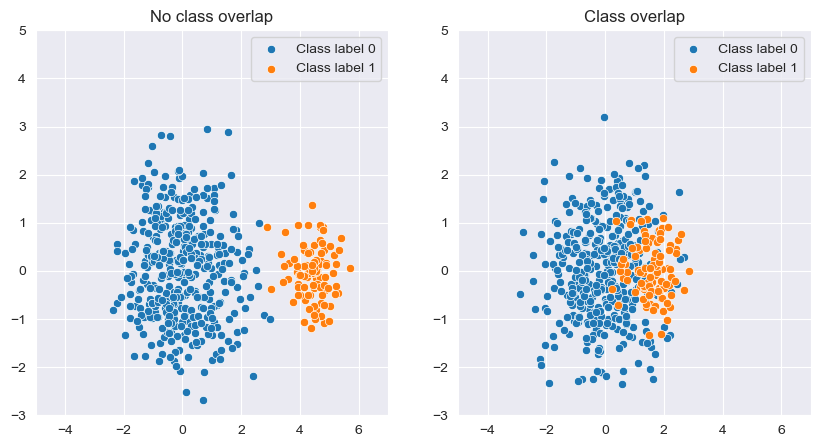
\includegraphics[width=\textwidth, height=140pt]{figures/related_work/classoverlap.png}
         \caption{Data uncertainty is higher when class overlap is present.}
     \end{subfigure}
     \hfill
     \begin{subfigure}[b]{0.49\textwidth}
         \centering
         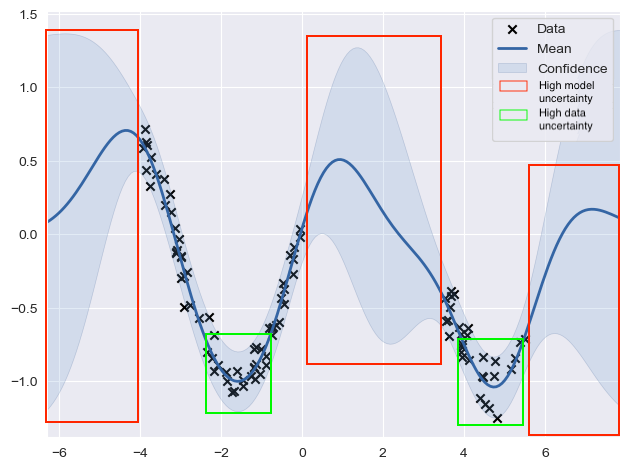
\includegraphics[width=\textwidth,height=140pt]{figures/related_work/gp.png}
         \caption{Difference between data and model uncertainty.}
     \end{subfigure}
     \caption{Data and model uncertainty.}
     \label{fig:data-mode-uncertainty-illustration}
\end{figure}

% explain UQ decomposition using heart-shaped data



Furthermore, in a text-generation application, the data uncertainty can be further divided into the following categories:
\begin{enumerate}
    \item Language uncertainty: the uncertainty of the language model itself, e.g. multiple different formulations can be used to express the same idea.
    \item Factual uncertainty: the uncertainty of the factual knowledge, e.g. in a question-answering use case, the model could answer incorrectly or even fabricate unrealistic answers, i.e. hallucinations.
    \item Input uncertainty: the uncertainty of the input data (prompt, context, etc.), e.g. the input could be noisy or contain errors. This is especially relevant for sequence-to-sequence or data-to-text models.
\end{enumerate}

\section{Calibration}

Machine learning models don't always produce reliable uncertainty estimates, e.g. classifiers are often over or under-confident regarding the SoftMax output probabilities. In addition, $\alpha$-confidence intervals might not cover the true value with an $\alpha$ probability.  % produced under wrong assumptions (e.g. normality, homoscedasticity, etc.)  
Poorly calibrated predictions negatively impact users who make informed decisions based on these predictions, especially in sensitive domain applications like healthcare. % talk about probability threshold. 
Model calibration is a post-training technique to adjust the predicted probabilities of a model so that they accurately reflect the true underlying probabilities of the events being predicted. True probabilities are estimated empirically using an extra dataset that is called the calibration dataset. Platt scaling\cite{platscaling}, Isotonic regression\cite{isotonicRegression}, and temperature scaling are common practical implementations of calibration. 

Calibration is often visualised using reliability diagrams (cf. figure \ref{fig:calibration-example}). In a binary classification task, the predicted probabilities of the true class are compared against the empirical class membership probabilities computed using the calibration dataset. Any deviation from the diagonal line is considered to be a calibration failure. Based on these plots, the area between the diagonal and the reliability curve is often used as a metric to assess the quality of an uncertainty quantification model.
%$P(c | score(x) = s)$
\begin{figure}
    \centering
    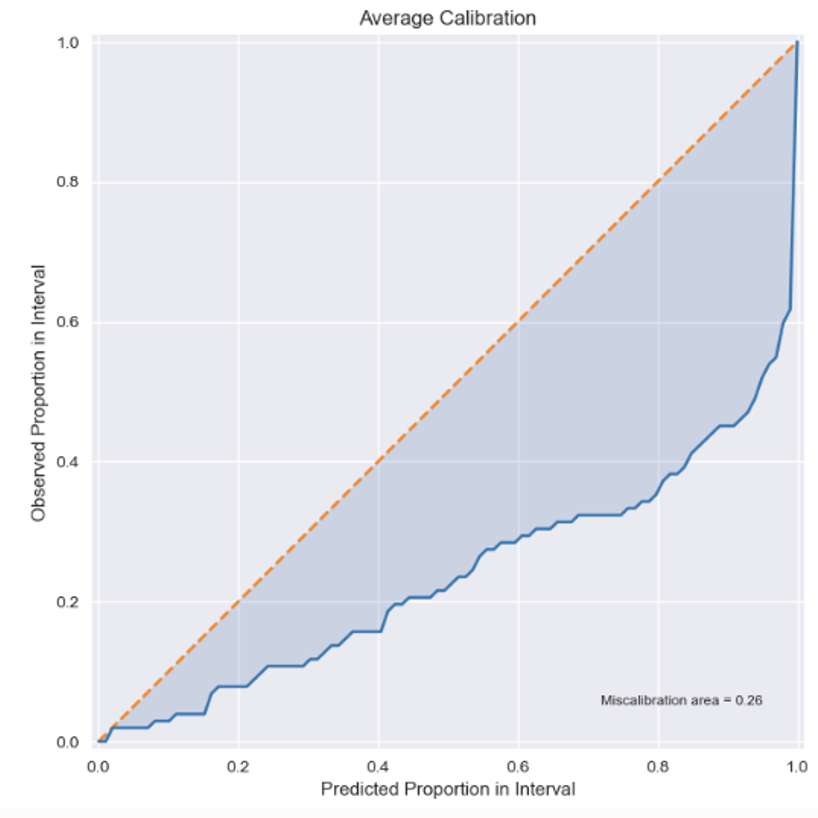
\includegraphics[scale=0.58]{figures/related_work/calibration.png}
    \caption{Example of reliability diagram for an under-confident model. The orange line represents a perfectly calibrated model. The data point (0.6,0.3) can be interpreted as follows: when the model predicts a 60\% probability of belonging to the true class, there is empirical evidence of 30\% in the calibration dataset that the prediction is a true positive.}
    \label{fig:calibration-example}
\end{figure}

Platt scaling is one of the most popular calibration methods and was initially introduced for support vector machine models. Consider a binary classification use case: given uncalibrated prediction probabilities for the true class label $\{ p_i \}_{i=1}^N$, Platt scaling optimises a parametric model based on the logistic function defined by
$$
f(p_i \mid A, B) = \Pb( y = 1 \mid p_i) = \frac{1}{1 + e^{- (A \cdot p_i + B)}}
$$
After training both parameters $A > 0$ and $B > 0$, the corrected probabilities are $\Tilde p_i = f(p_i)$.

In contrast, isotonic regression is a non-parametric regression over the class of non-decreasing (i.e. isotonic) functions, i.e. $\forall_{i,j}$ if $ p_i \leq p_j$ then $\Tilde p_i \leq \Tilde p_j$. The Pair-adjacent violators (PAV) algorithm is commonly used to fit an isotonic stepwise-constant function $I$ by optimising the mean-square error criterion. The isotonic property of the mapping function enforces the same probability ranking before and after applying the function. Due to its non-parameter nature, it usually requires more training data than Platt scaling and is more prone to overfitting.

Finally, temperature scaling (TS) is a single-parameter variation of the Platt Scaling approach. It rescales logit scores by a parameter $T$ before applying the SoftMax function $SoftMax(f_i / T) $ to better match the empirical class membership probabilities. TS is straightforward yet effective while maintaining a low memory complexity to calibrate machine learning models, also in the case of deep neural networks\cite{TSDeepNets}.

% (a) show calibration picture.


\section{Bayesian learning}

Bayesian learning takes a different approach than traditional frequentist machine learning to perform statistical inference by modelling a complete distribution over possible parameters of the model instead of point estimates. At its core, Bayes' theorem allows the incorporation of prior information about the model parameters into the prediction process. Let $D_{train} = \{X,Y\}= \{(x_i,y_i)\}_{i=1}^N$ be the training set so that $x_i \in \R^D$ and $y_i \in \R$ or $y_i \in \{1,\ldots,C\}$ depending on whether the application is a regression or a classification. Bayesian learning aims to optimise the weights $\theta$ of the model $f_\theta(\cdot)$ using the posterior distribution 
$$
\Pb(\theta \mid X, Y) 
= \frac{\Pb(Y \mid X, \theta) \cdot \Pb(\theta) }{\Pb(Y \mid X) }
\propto Likelihood \, \times \, Prior
$$

The complexity of this operation depends on the marginalisation step, which cannot be computed analytically in most real-life scenarios:
$
\Pb(Y \mid X) = \int \Pb(y \mid x, \theta) \cdot \Pb(\theta \mid X,Y) \;d\theta
$.


To address this issue, variational approaches propose to approximate $\Pb(\theta \mid X, Y)$ using variational parameters $q_\omega(\theta)$ so that the Kullback–Leibler divergence between both distributions, $KL(q_\omega(\theta) \parallel \Pb(\theta \mid X, Y) )$, is minimised with respect to $\omega$. 
The Bayesian counterpart of neural networks, Bayesian Deep Learning (BDL) and Bayesian NNs (BNNs), are popular methods to interpret the model parameters and produce insights about their reliability without overfitting the data. Tools such as Monte Carlo (MC) dropout\cite{dropoutDeepNets}, Markov chain Monte Carlo (MCMC) or Variational inference (VI) are used to approximate the posterior inference. Multiple estimates for the target variable can be produced via a sampling procedure over the weight distribution, which can be turned into an uncertainty score.
 

\section{Ensembles} \label{section:background:ensembles}

Ensemble learning is a machine learning tool that trains multiple different predictors and combines their results into a final prediction. Ensembles aim to reduce the model's variance and produce more accurate and robust predictions than any of the underlying predictors, which can be prone to over-fitting or under-fitting the training data. 
One of the most popular methods to combine these predictions is to take their simple average. However, other methods exist, such as taking the median or the weighted average, which puts more influence on specific models.
Ensembling is a very popular technique used in a wide range of applications. Many popular algorithms, such as Random Forests, are based on this principle. They also have major implications in the uncertainty quantification field, as shown in section \ref{model:uq-ensembles}.



% other question how to create the ensemble?
% discrete and finite set of learners => if infinite => tend to bayesian learning.
% variance reduction => improve bias-variance tradeoff
% In the literature, ensembles are often used to predict the mean and not variance

\section{Adversarial machine learning}

Along with the widespread of machine learning in day-to-day use, such as medical applications or self-driving cars, there has also been a growing concern for security and robustness in these systems. Interestingly, it turns out that many of the top-performing models are vulnerable to what are called adversarial examples. These are crafted inputs which may be indistinguishable from original inputs to human eyes and yet have been specifically designed to cause a failure for the model to classify them correctly.
Therefore, adversarial machine learning aims to deceive or mislead the model or person relying on its predictions using attacks and to learn how to defend against them. 

%%%%%%%%%% survey paper on adversarial ML
Nowadays, various threat models and adversaries can be exploited by attackers to attempt to break these models. Still, only a limited number of countermeasures are available to act against them. Defence is articulated around two pillars: attack detection to filter them before they enter the system and special training to make models more robust against them. On the attack side, adversarial examples can be generated, for instance, using optimisation-based methods. One widely known attack is the fast gradient sign method (FGSM)\cite{FGSM} that leverages the gradient of the loss function with respect to the input data to create small perturbations that are then turned into adversarial examples. This attack is fast and powerful since it can be computed efficiently using back-propagation in the case of neural networks.

\section{Knowledge Graphs}
\say{
A knowledge graph mainly describes real-world entities and their interrelations, organised
in a graph\cite{KnowledgeGraphDef}.}. Even though more formal definitions have been proposed\cite{KnowledgeGraphDefFormal}, this simple definition covers the needs of this work. Knowledge graphs are often represented in the Resource Description Format (RDF), i.e. into a set of triplets. Triples encode edges of the graph in a subject-predicate-object format such as \textit{(John, is friend with, Bob)}. 

% Idea: DBPedia dataset 

\section{Natural Language Processing}

Natural Language Processing (NLP) focuses on the relationship between human language and computer systems. It is an interdisciplinary domain at the intersection of linguistics, computer science and artificial intelligence. In particular, NLP aims to build algorithms capable of understanding and extracting pieces of information from a text corpus or generating human-like texts. The latter tasks are the concentration area of this thesis regarding NLP. The following sections introduce the necessary concepts to understand chapter~\ref{chatper:design}.

\subsection{Named-Entity Recognition}

Named-Entity Recognition (NER) is the process of identifying and classifying entities in unstructured texts. Usually, a fixed set of entities are considered, e.g. organisations, person names, time and dates, quantities, etc. An example of NER output is shown below (\href{https://tdai.osu.edu/sites/default/files/2022-06/2022-foundations-tutorial3-sunwang-deeplearning4nlp.pdf}{source}):

\begin{center}
    Ousted [WeWork]\textsubscript{Organisation} founder [Adam Neumann]\textsubscript{Person} lists his [Manhattan]\textsubscript{Location} penthouse for [\$37.5 million]\textsubscript{Amount}.
\end{center}

First, different entities can be identified, i.e. localised in the text: \textit{WeWork}, \textit{Adam Neumann}, \textit{Manhattan} and \textit{\$37.5 million}. Then, they can be classified further into the following categories: \textit{organisation}, \textit{person}, \textit{location} and \textit{amount}. This two-step procedure is a common abstraction of the NER task. However, many practical implementations, such as the state-of-the-art transformed-based models, do not follow this structure. More formally, each named entity $NE_i$ in a text $T = \{t_1,\ldots,t_n\}$ composed of $n$ tokens is defined by a triple $NE_i= (s_i, e_i, c_i)$ where $s_i, t_i \in \{1, \ldots, n\}$ respectively represent the start and end index of the entity in the text. $c_i$ corresponds to one of the predefined entity types. %discuss evaluation if needed.

\subsection{Transformers}

Transformers are a type of neural network architecture introduced in 2017\cite{transformers} based on the concept of self-attention to construct contextualised word embeddings. 
Transformers have grown in popularity ever since and now serve as a reference point for many NLP tasks such as machine translation, text classification or language generation. One of the key benefits of this architecture is its ability to process larger amounts of text efficiently and better exploit long-range dependencies in the input text compared to other models such as RNNs or LSTMs. 
% explain how pretraining-fine tuning works
These models have also popularised the concept of transfer learning, i.e. pre-training and fine-tuning. In the first phase, they are trained using a self-supervised procedure on a large corpus of unannotated text usually taken from the Web. The training task differs from one model to another, but the most simple one is to predict the next work in a sequence given the previous ones and is known as language modelling. BERT\cite{BERT} uses a slight variation called masked-language modelling (MLM) that predicts masked words:

\epigraph{
The boy walked to the store, but he realised he forgot his \textbf{[MASK]} on the kitchen table.
}{Example of a masked language modelling input}
\newpage
In the second fine-tuning phase, the model is adapted to a downstream task using a considerably smaller dataset than the pre-training corpus. Fine-tuning is about harvesting the language information stored during pre-training and slightly updating the weights better to match the vocabulary and style of the downstream task.   
% focus on transformer architecture
The original transformer used an encoder-decoder architecture. The input is processed by a series of encoding layers that extract information about which parts of the input are relevant to the others. The decoder takes a reversed approach and starts from the contextualised word representations created by the encoder to reconstruct a sequence of tokens as output. Both components operate using an attention mechanism that can be decomposed into scaled dot-product attention units. Each unit learns three weight matrices to  produce embeddings for every token:  the query weights $W_{Q}$, the key weights $W_{K}$, and the value weights  $W_{V}$. Given $X$, the matrix containing word embeddings as rows, $Q = X \cdot W_Q$, $K = X \cdot W_K$ and $V = X \cdot W_V$, the attention scores $A$ can be computed as follows

$$
A = Softmax \left(\frac{Q \cdot K^T}{\sqrt{d_k}} \right) V
$$
where $\sqrt{d_k}$ is a gradient stabilisation factor during training. 

% to be paraphrased 
% The final word embedding not only contain information about the word itself but also a combination of other tokens, each weighted by its attention weight

At inference time, transformers rely on decoding algorithms to produce human-like text. The most straightforward one is greedy decoding which is fast but tends to deliver redundant and dull outputs\cite{issuesDecodingSamplingNLP}. At each step, the highest probability token given the previously generated ones is selected. This causal procedure is repeated until some desired length is reached or an end-of-sequence token is generated. Beam search decoding has been proposed to offer more diverse and probable sequences. It maintains a buffer of the $B$ most probable sequences generated so far, i.e. the beams. At each step, each of these beams explores the next $B$ most probable tokens which result in $B^2$ possible candidates. Those with the lowest joint probability are pruned so that only the top $B$ candidates remain. As the beam size $B$ increases, beam search becomes slower to execute with a lower bound at $B=1$, i.e. greedy search. Alternatively, stochastic text generation approaches utilise the token probability distribution to sample the tokens at each step to avoid generic outputs. Random sampling is a simple strategy but tends to produce several rare tokens and, thus, unrealistic text. To address this issue, different sampling variations have been introduced to cut-off probability mass for unlikely tokens. Top-K sampling exclusively considers the K most probable tokens. In contrast, nucleus sampling\cite{nucleusSampling} is based  on Top-$L$ sampling where $L$ is the smallest integer so that the cumulative probability distribution for these $L$ tokens exceeds some probability threshold $p$.



% conclusion before next section
Part of their success can also be attributed to the open-source access of pre-trained implementations, e.g. the BERT-family of models created by HuggingFace. In this thesis, specific focus has been directed to the text-to-text transfer transformer or T5\cite{T5}.

\subsection{T5 and sequence-to-sequence models}

Sequence-to-sequence models are based on the encoder-decoder architecture and are used to transform one sequence into another where input and output can be of arbitrary length. The goal of the encoder is to create a fixed-length numeral representation of the input sequence, %, i.e. the last hidden state, 
which is then passed to the decoder. The decoder leverages this information as part of the auto-regressive output sequence generation to produce input-dependant tokens.

T5 or the text-to-text transfer transformer\cite{T5} is an example of the sequence-to-sequence architecture. As opposed to the BERT-family of models that can only return a class label or a span of the input,  T5 is, at its essence, a standardised proposal to represent all NLP tasks in a text-to-text format. In other words, the same model, loss function and hyper-parameters are used to simultaneously train heterogeneous tasks such as machine translation, question answering, sentiment analysis, etc. The pre-training objective of T5, i.e. sized-fill-in-the-blank text generation, differs from BERT's MLM because the model is asked to fill an approximate number of words at some specific place in the sentence, which can also be at the end. For example, given as input the string \textit{"I like to eat peanut butter and \_4\_ sandwiches"}\cite{googleBlogT5}. The model could fill the blank using the sequence: \textit{"jelly, which is what makes good"} while a size-2 masked token \textit{\_2\_} would result in \textit{"jelly on my"}.



% T5 pre-training task from google
% https://ai.googleblog.com/2020/02/exploring-transfer-learning-with-t5.html


\subsection{Graph-to-text and text-to-graph} \label{background:G2T}

% data2text models are prone to hallucinations compared to template-based models\cite{challengesData2Text}


% into what is a graph to text and goals
The graph-to-text generation task aims to convert structured information given as a graph into a fluent textual output. On the other end, text-to-graph is the converse task of extracting relevant entities from the input text, i.e. nodes, and the relationships between them, i.e. edges. Graph-to-text models can be used for a variety of tasks, including question-answering, content generation, etc. In contrast, text-to-graph models are more applicable to data-mining or information extraction.
%different pipeline approach
Consider an example from the WebNLG dataset: the graph is shown in table \ref{table:example:graph}, and the reference text is:

\epigraph{
Alan Bean was an American astronaut, born on March 15, 1932, in Wheeler, Texas. He received a Bachelor of Science degree at the University of Texas at Austin in 1955 and was chosen by NASA in 1963.
}{Reference text}

\begin{table}[ht]
\centering
\caption{Graph example from WebNLG dataset in RDF format.}
\label{table:example:graph}
\begin{tabular}[t]{llll} % p{3cm}
\hline
 &  Subject & Relation & Object \\
\hline
1& Alan Bean & nationality & United States \\
2& Alan Bean & birth date   & 1932-03-15    \\
3& Alan Bean & alma mater   & UT Austin, B.S. 1955 \\
4& Alan Bean & birth place  & Wheeler, Texas \\
5& Alan Bean & selection   & 1963 \\
\hline
\end{tabular}
\end{table}%



% currently 

As of today, state-of-the-art models are built using sequence-to-sequence transformers such as T5. As a result, the graph must first go through a linearisation process to be transformed into a sequential textual representation that can then be fed to the model for training. Special tokens $<H>$, $<R>$ and $<T>$ are added to the tokenizer of the model to put emphasis respectively on the start of the subject, relation and object part of each edge. After concatenating all edges one after the other, the linearised example graph becomes:

\epigraph{
<H> Alan Bean <R> nationality <T> United States
<H> Alan Bean <R> birth date <T> 1932-03-15
<H> Alan Bean <R> alma mater <T> UT Austin, B.S. 1955 
<H> Alan Bean <R> birth place <T> Wheeler, Texas
<H> Alan Bean <R> selection <T> 1963
}{linearised graph}

% explain 
The linearised graph and text pairs are then used to fine-tune two independent T5 models, one for graph-to-text and one for text-to-graph. Even though this approach generates highly performing models, the linearisation phase has been criticised in the literature due to its inability to exploit the structural properties of the graph. Models such as JointGT\cite{JointGT} have been proposed to improve the encoding phase of the transformer. However, they are not considered in this thesis work. 

%In addition, manual data collection and labelling is often a tedious process for these models, resulting in scarce training datasets. To overcome this issue, an unsupervised approach, CycleGT\cite{cycleGT}, was introduced in 2020. It trains both graph-to-text and text-to-graph pipelines in rounds with unpaired text and graph datasets. It has been shown to reach comparable performance to supervised counterparts.



